%%%%%%%%%%%%%%%%%%%%%%%%%%%%%%%%%%%%%%%%%%%%%%%%%%%%%%%%%%%%%%%%%%
%%%%%%%% ICML 2016 EXAMPLE LATEX SUBMISSION FILE %%%%%%%%%%%%%%%%%
%%%%%%%%%%%%%%%%%%%%%%%%%%%%%%%%%%%%%%%%%%%%%%%%%%%%%%%%%%%%%%%%%%

% Use the following line _only_ if you're still using LaTeX 2.09.
%\documentstyle[icml2016,epsf,natbib]{article}
% If you rely on Latex2e packages, like most moden people use this:
\documentclass{article}

% use Times
\usepackage{times}
% For figures
\usepackage{graphicx} % more modern
%\usepackage{epsfig} % less modern
\usepackage{subfigure} 

% For citations
\usepackage{natbib}

% For algorithms
\usepackage{algorithm}
\usepackage{algorithmic}
\usepackage{amsfonts}
% As of 2011, we use the hyperref package to produce hyperlinks in the
% resulting PDF.  If this breaks your system, please commend out the
% following usepackage line and replace \usepackage{icml2016} with
% \usepackage[nohyperref]{icml2016} above.
\usepackage{hyperref}

% Packages hyperref and algorithmic misbehave sometimes.  We can fix
% this with the following command.
\newcommand{\theHalgorithm}{\arabic{algorithm}}

% Employ the following version of the ``usepackage'' statement for
% submitting the draft version of the paper for review.  This will set
% the note in the first column to ``Under review.  Do not distribute.''
\usepackage{icml2016} 

% Employ this version of the ``usepackage'' statement after the paper has
% been accepted, when creating the final version.  This will set the
% note in the first column to ``Proceedings of the...''
%\usepackage[accepted]{icml2016}


% The \icmltitle you define below is probably too long as a header.
% Therefore, a short form for the running title is supplied here:
\icmltitlerunning{Bi-Directional Generative Recurrent Adversarial Networks}

\begin{document} 

\twocolumn[
\icmltitle{ Bi-Directional Generative Recurrent Adversarial Networks}

% It is OKAY to include author information, even for blind
% submissions: the style file will automatically remove it for you
% unless you've provided the [accepted] option to the icml2016
% package.
\icmlauthor{Benjamin Striner}{bstriner@andrew.cmu.edu}
\icmladdress{Your Fantastic Institute,
            314159 Pi St., Palo Alto, CA 94306 USA}

% You may provide any keywords that you 
% find helpful for describing your paper; these are used to populate 
% the "keywords" metadata in the PDF but will not be shown in the document
\icmlkeywords{boring formatting information, machine learning, ICML}

\vskip 0.3in
]

\begin{abstract} 
We present a Bi-Directional Generative Recurrent Adversarial Network (BiGRAN) that is able to encode and decode recurrently. BiGRAN is an extension of GRAN, which is able to iteratively generate samples but does not include an encoder \cite{Im2016}. BiGRAN is also an extension of BiGAN, which jointly trains an encoder and generator\cite{Donahue2016} but has not yet been adapted to a recurrent setting. A BiGRAN can autoencode and generate samples from the MNIST dataset and iteratively constructs samples. Recent work on generative models have included methods of attention and iterative improvement \cite{Gregor2015, Makhzani2016, Denton2015, Sønderby2016}. BiGRANs provide a framework that would allow extension with attentive mechanisms as in the DRAW model \cite{Gregor2015}. We also present recurrent discrimination, an implementation of minibatch discrimination using recurrent networks.
\end{abstract} 

\section{Introduction}
\label{introduction}

Generative Adversarial Networks (GANs) provide a framework for training a model to generate samples from an input distribution. However, GANs do not provide a means of learning the inverse function, encoding, mapping samples from an input distribution to a latent distribution. Bi-Directional Generative Adversarial Networks (BiGANs) provide a framework by which both generator and encoder can be trained by a single discriminator. 

We propose and experiment with Bi-Directional Generative Recurrent Adversarial Networks (BiGRANs) to train a model that can both encode and generate in a recurrent fashion. Our BiGRAN iteratively generates a sample by summation into a canvas, similar to the DRAW model \cite{Gregor2015}. The discriminator is trained on samples from each time step. As such, the encoder and generator receive reinforcement at each time step and learn to iteratively correct generated samples.

The DRAW model is structured around VAEs. VAEs assume some reconstruction loss such as mean squared error or binary cross entropy. It would be advantageous to provide a similar formulation to DRAW built using an adversarial model.

We also present experiments with recurrent discrimination. Recurrent discrimination is a type of minibatch discrimination utilizing recurrent networks. Minibatch discrimination is a strategy by which a discriminator views several samples instead of a single sample. By allowing the discriminator to consider several samples, the discriminator is better able to reject samples due to lack of variance, which increases the variance in the generated samples.

\section{Related work}

Generative Adversarial Networks (GANs) learn a generative model that maximally confuses a descriminator trained to descriminate between generated and real samples \cite{Goodfellow2014}. There are several models closely related to GANs. An example is Conditional Generative Adversarial Networks that model a conditional distribution \cite{Mirza2016}.


$$ \min_G \max_D V(D,G) $$
$$ V(D,G) = V_D(D) + V_G(D,G) $$
$$ V_D(D) = \mathbb{E}_x [\log(D(x))] $$
$$ V_G(D,G) = \mathbb{E}_z [\log(1-D(G(z)))] $$

\subsection{BiGANs}

Bi-Directional Generative Adversarial Networks (BiGANs) \cite{Donahue2016} provide an architecture by which an adversarial model can learn both encoding and decoding. VAEs are generative models that perform autoencoding. In contrast to VAEs, GANs are typically one-way-streets; GANs allow generation of samples but not encoding samples to a representation in the latent space.

The minmax objective of a BiGAN is similar to a GAN but includes minimization over both a generator $G$ and encoder $E$. This allows the model to learn a pair of symmetric functions in an adversarial fashion.

$$ \min_{G, E} \max_D V(D,E,G) $$
$$ V(D,E,G) = V_E(D, E) + V_G(D, G) $$
$$ V_E(D,E) = \mathbb{E}_{x}[ \log D(x, E(x))] $$
$$ V_G(D,G) =  \mathbb{E}_z[ \log(1-D(G(z),z))] $$

\subsection{GRANs}

The Generative Recurrent Adversarial Network (GRAN) \cite{Im2016} provides a model in which the generator of a GAN is recurrent. The generator receives a series of samples from the latent space and outputs a series of samples that are summed into a canvas. The canvas generates samples in the target distribution. 

This model allows iterative generation instead of attempting to generate an entire image all-at-once. Iterative generation allows for more complicated generation such as attentional methods.

\subsection{Minibatch discrimination}

A common failure mode of GANs is to underestimate the variance of the data. In practice, a common failing is to emit variations of only one or a few numbers, as shown in Figure \ref{fig:failures}. As shown in Figure \ref{fig:gan}, failure is extremely sensitive to learning rate, batch size, and model complexity.

An approach to avoid collapse is \textit{minibatch discrimination} \cite{Salimans2016}. In minibatch discrimination, the discriminator receives side-information regarding other samples within the minibatch. This side-information enables the discriminator to better reject samples due to a lack of variance. Specifically, the approach in  \cite{Salimans2016} provides side-information regarding the average L1 difference of feature vectors within the minibatch. 

\begin{figure}[h]
\caption{A common failure mode of GANs that are not sized or trained correctly is to emit only a subset of the population. Two trials of the same model collapse to a different subset of the space each time. }
\label{fig:failures}
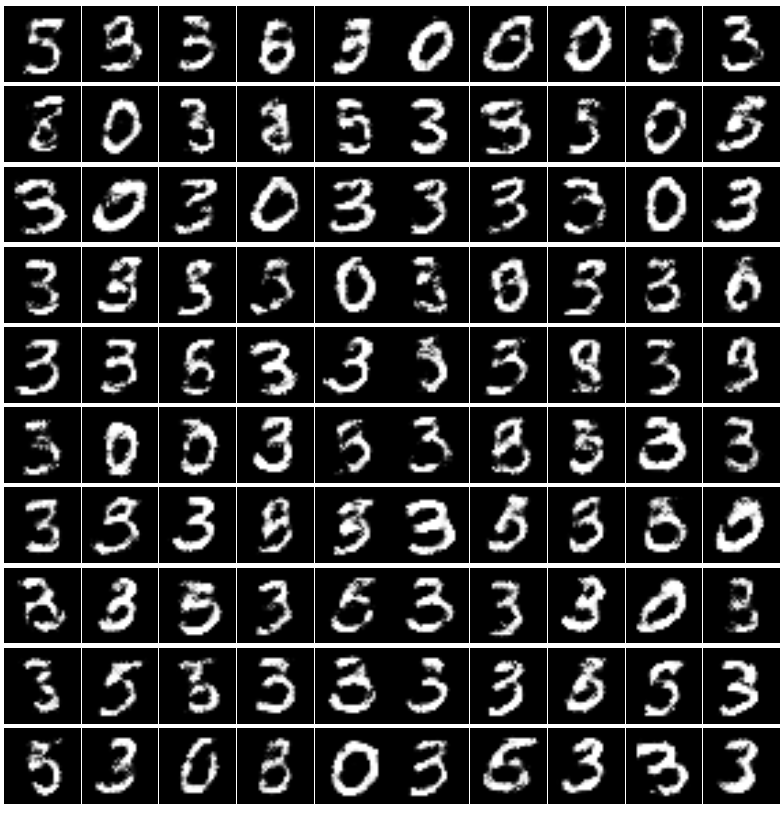
\includegraphics[scale=0.3]{images/failure1.png}
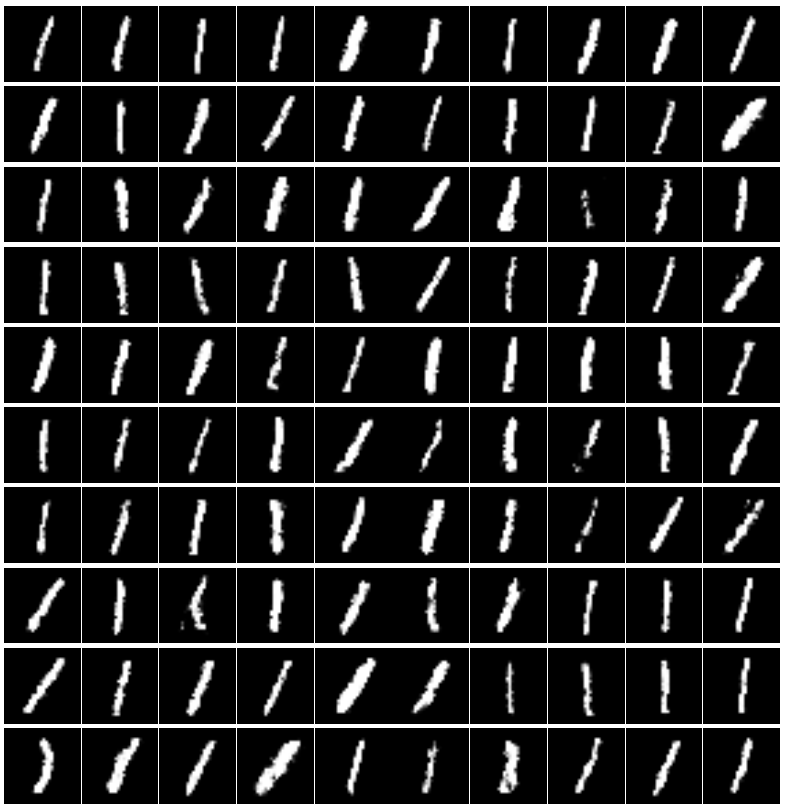
\includegraphics[scale=0.3]{images/failure2.png}
\centering
\end{figure}
\begin{figure}[h]
\caption{Same model as Figure \ref{fig:failures} with adjusted learning rate and batch size, which converges to better approximate the true variance. }
\label{fig:gan}
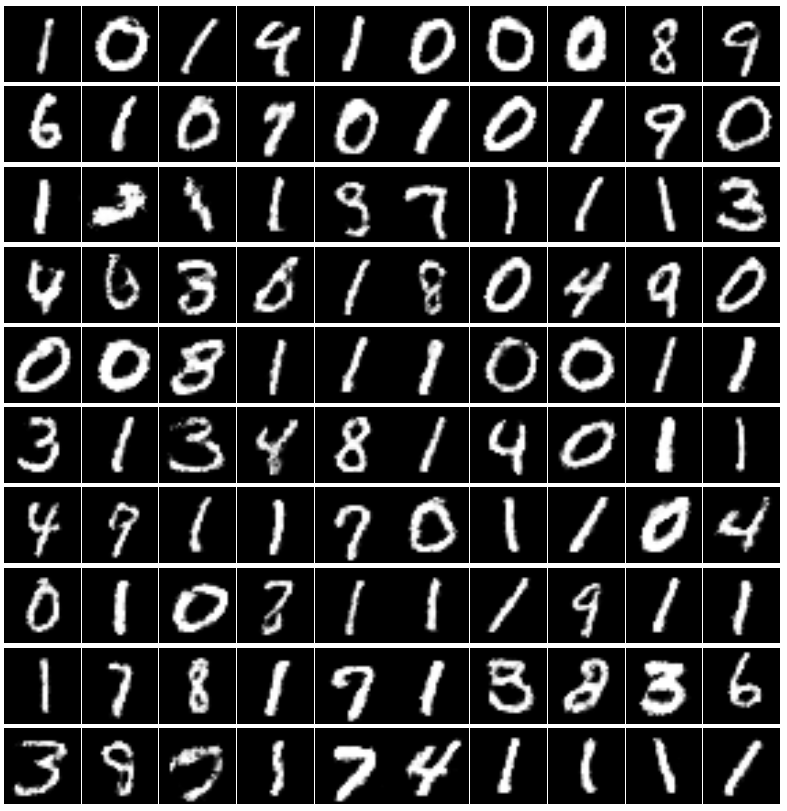
\includegraphics[scale=0.3]{images/success.png}
\centering
\end{figure}

\subsection{Variational Autoencoders (VAEs)}



Variational Autoencoders (VAEs) are models in which a stochastic autoencoder is trained with the hidden representations regularized towards some prior distribution \cite{Doersch2016}. VAEs analytically solve for the KL divergence between samples from the hidden layer and some prior, and include that divergence in the objective function. The hidden representations are drawn from a distribution that is easy to sample from. The model can generate samples by sampling from the hidden space and decoding that hidden representation.

The Adversarial Autoencoder (AAE) \cite{Makhzani2016} is similar to a VAE, but the hidden representations are regularized adversarially instead of by minimizing the KL divergence. A descriminator is trained to predict whether hidden activations are drawn from a prior distribution or the model. This regularizes the hidden representations of the autoencoder towards some prior, typically a Gaussian, but any prior that can be sampled from can be used. 

The Deep Recurrent Attentive Writer (DRAW) model shows promising results using an attentional mechanism and iterative improvements \cite{Gregor2015}. A VAE both learns a difference image and to control an attention mechanism.

Ladder Variational Autoencoders (LVAEs) recursively correct the generative distribution \cite{Sønderby2016}. Future work could attempt to construct a ladder BiGAN in a similar manner.

%%Theis discusses the issues with evaluation of generative models \cite{Theis2016}. It is important to evaluate models through a variety of methods including log-likelihood and evaluation of samples. Theis demonstrates that high-quality samples and high log-likelihood are independent.
%%Denton presents a model in which an image is decomposed into a Laplacian / Difference-of-Gaussians pyramid \cite{Denton2015}. A GAN is trained to generate each level of the pyramid, conditioned on the previous level. The model is trained on CIFAR10 and LSUN.


\section{Recurrent discrimination}
Minibatch discrimination works for intuitive reasons. Consider the failures presented in Figure \ref{fig:failures}. Suppose that a GAN learns to perfectly produce only the number ``1''. The probability of that number under the true distribution is $0.1$ and the probability under the generated distribution is $1.0$. The number ``1'' is 10 times more frequent in the generated distribution than the true distribution.

Given one ``1'', the likelihood under the true distribution is $0.1$ and the likelihood under the generated distribution is $1.0$. Given two ``1''s, the likelihood under the true distribution is $0.01$ and the likelihood under the generated distribution is $1.0$. Given a larger number of samples, there is a greater difference between the true and generated distributions. Allowing a discriminator to view multiple samples would allow the discriminator to better reject samples due to lack of variance.

Minibatch discrimination may be implemented using recurrent networks, a method we will call recurrent discrimination. We present experiments with recurrent discrimination on a toy problem and a simple GAN and then apply recurrent descrimination to our BiGRAN.

\subsection{Toy recurrent discrimination}
In a simple example, we consider a discrete input space of 10 categories. We construct a toy generator to experiment with mode collapse.

The true population has an equal probability $p=0.1$ for each category. The toy generator generates the first five categories with equal probability $p=0.2$ and does not generate the second five, such as would occur in a failing GAN.

We train a recurrent discriminator and compare the output of the discriminator with varying depths. The discriminator network is implemented as a dense layer with sigmoid activation on top of an LSTM. The LSTM sequentially receives either samples from the generator or samples from the true distribution. The objective function is binary crossentropy, which is minimized when the output of the discriminator is the true probability of the sample being drawn from the true distribution.

Given that the first five categories are twice as likely in the toy distribution than the true distribution, the probability that a set of samples comes from the true distribution is $\frac{p^k}{1+p^k}$ where $k$ is the number of samples and $p=0.5$. This reflects that as the number of samples grows larger, there is greater confidence that those samples come from the toy distribution, with decreasing returns. With an infinite number of samples, a discriminator can discriminate perfectly.

$$ D_k(x) = \frac{p(x)^k}{1+p(x)^k}$$

As shown in Figure \ref{table:rd}, a recurrent discriminator is able to accurately learn the probability of sets of varying number of samples. Samples from the generator are rejected more strongly as a function of the number of samples, with decreasing marginal returns. Increasing the number of samples considered in minibatch discrimination should yield decreasing returns but increasing the number of samples will likely increase complexity linearly.

\begin{figure}[h]
\caption{Function learned by LSTM matches likelihood function. Recurrent discriminators reject samples due to lack of variance with decreasing marginal returns on number of samples.}
\label{table:rd}
\centering
\begin{tabular}{ l l l } 
 \hline  \hline
 Depth (k) & Discriminator Output & $\frac{p^k}{1+p^k}$ \\
 \hline
 1 & 0.3363147 & 0.33333 \\
 2 &  0.1982634 & 0.20000 \\
 3 &  0.1088916   & 0.11111 \\
 4 &  0.0486446 & 0.05882 \\  \hline  \hline
\end{tabular}
\end{figure}

\subsection{MNIST recurrent discrimination}
In a more complicated example, we train a simple GAN to generate MNIST digits. We utilize recurrent discrimination and vary the depth of the discriminator to examine results on the generated samples.

The generator is a network with two tanh hidden layers and a sigmoid output layer. The discriminator is an LSTM that feeds a fully connected layer with a sigmoid output.

As shown in Figures \ref{fig:rd1}, \ref{fig:rd2} and \ref{fig:rd4}, increasing the depth of the recurrent discriminator increases the variance of the generated samples. Early in training, the depth of the discriminator corresponds to the number of modes of the generator.

\begin{figure}[h]
\caption{After 10 epochs, recurrent discrimination with $k=1$ is a typical GAN and prone to collapse.}
\label{fig:rd1}
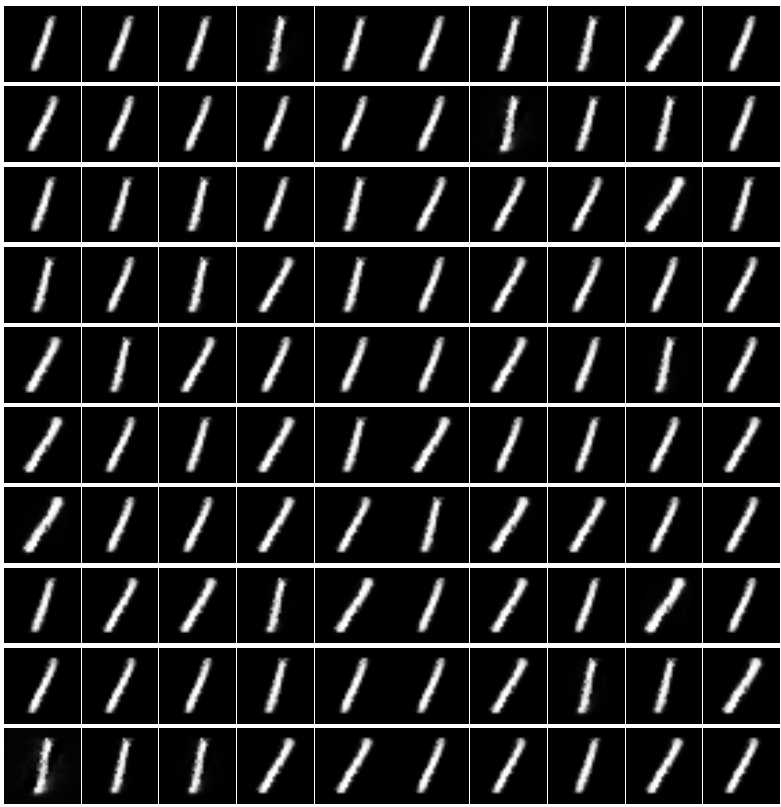
\includegraphics[scale=0.3]{images/minibatch1.png}
\centering
\end{figure}
\begin{figure}[h]
\caption{After 10 epochs, recurrent discrimination with $k=2$ forces the generator to emit multiple modes.}
\label{fig:rd2}
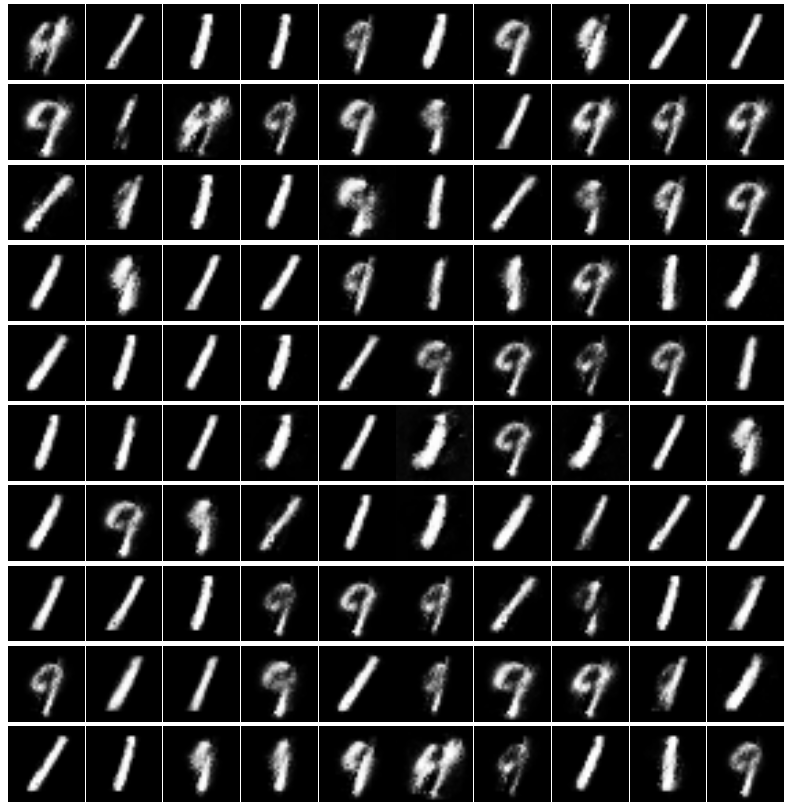
\includegraphics[scale=0.3]{images/minibatch2.png}
\centering
\end{figure}

\begin{figure}[h]
\caption{After 10 epochs, recurrent discrimination with $k=4$ further increases variance.}
\label{fig:rd4}
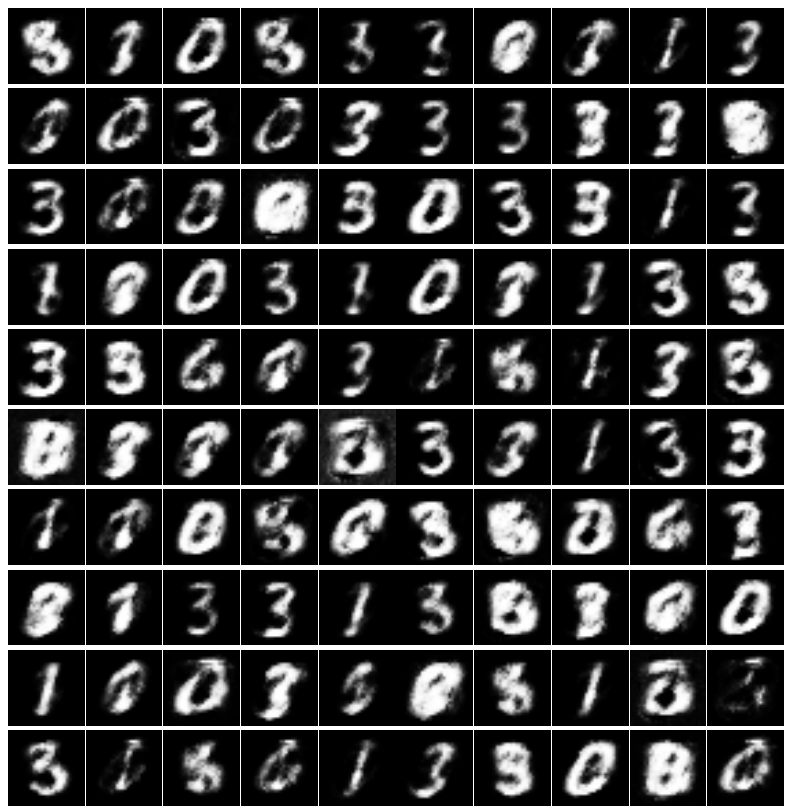
\includegraphics[scale=0.3]{images/minibatch4.png}
\centering
\end{figure}

%\section{Squared Hinge Loss}

%Typically, GANs are trained using a sigmoid output layer, such that the discriminator attempts to assign 0 to fake samples and 1 to real samples, and the network is trained by binary cross-entropy \cite{Goodfellow2014}. This architecture leads to easy probabilistic interpretation. Another similar architecture is to train a softmax output layer with 2 categories.

%We propose and experiment with training GANs using linear output layers and squared hinge loss.

%$$ L(y, \hat{y}) = \max(0, 1- (y \hat{y})^2)$$

%Squared hinge loss has the property that if $y=1, \hat{y} \ge 1$ or $y=-1, \hat{y} \le -1$, the loss is 0. In contrast, a sigmoid output can never reach 0 or 1, so always has some nonzero loss.

%Another common failure mode of GANs is to not learn or learn very slowly. If the discriminator learns too much, the output for generated samples will be squashed, and very little gradient will be available to train the discriminator. On the other hand, the generator only learns through the discriminator, so it is important that the discriminator learns faster than the generator. As such, there is a careful ballance between the discriminator making enough of a distinction that the generator can learn, but not so much that the gradient is completely squashed.

%Using a sigmoid or softmax output leads to the gradient being squashed if the discriminator overlearns. Hinge loss and squared hinge loss share the property that even if the discriminator is trained until it has 0 loss, there will be large gradient by which to train the generator.
 
%Utilizing hinge loss does not lend to an easy probabilistic interpretation but that concern comes secondary to model performance. We provide experiments showing that squared hinge loss is more resistant to discriminator overlearning.

%\{Add discussion of energy-based GANs\}

\section{BiGRAN Model}
 
We experimented with a BiGRAN on the MNIST dataset. The foundation of the model is the Bi-Directional Generative Adversarial Network (BiGran) \cite{Donahue2016} and Generative Recurrent Adversarial Network  (GRAN) \cite{Im2016}. This model trains a recurrent encoder, decoder and discriminator. \footnote{For implementation details, see source code at \url{https://github.com/BenStriner/bigran}.}
 
Let $n$ be the input dimension,  $m$ be the latent dimension, $k$ be the recurrent depth, $x$ be input samples and $z$ be latent samples.
 
 \subsection{Encoder}
 
 The encoder is an LSTM that view the input and generates a series of samples in the latent space. The encoder is a stochastic network created using the reparameterization trick. The outputs of the encoder network are linear activations interpreted as the $\mu$ and $\log \sigma^2$ of the embedding in latent space. The embeddings are then created by sampling $\epsilon$ from a unit Gaussian and applying the reparameterization trick. L1 weight regularization is applied to the encoder.
 
$$\mu + \epsilon e^{\frac{\log \sigma^2}{2}} = \mu + \epsilon \sigma$$

\subsection{Decoder}
 
The decoder is an LSTM that processes a series of samples from the latent space and emits samples in $R^n$ with linear activation. These samples are cumulatively summed into a canvas. A sigmoid activation is applied to convert the canvas into generated samples in the same space as the target samples. L1 weight regularization is applied to the decoder.

\subsection{Discriminator}

The discriminator is composed of several parts. A subnet processes samples from the latent space, a subnet processes samples from the target space, and a subnet combines information across samples. L1 weight regularization and dropout are applied to the discriminator.

An LSTM processes the samples from the latent space, iterating over sequential encodings.

A two layer tanh network processes the samples from the input space.

Hidden representations from the latent space and input space are concatenated.

An LSTM processes the hidden representations, iterating over different samples.
 
In contrast to the GRAN, our recurrent networks are connected at each time step. The discriminator is trained to discriminate generated samples at all timesteps $1...k$. Gradient from the discriminator is propagated to the output of the generator and discriminator at all timesteps both through the final timestep and through all intermediate timesteps.

\section{Results}

The BiGRAN learns to generate and autoencode digits from the MNIST dataset. 

Figure \ref{fig:generated} shows images randomly generated from the BiGRAN.
 
\begin{figure}[h]
\caption{Samples drawn from BiGRAN with pairwise discrimination. Show better variance than without pairwise discrimination but still underestimate true variance.}
\label{fig:generated}
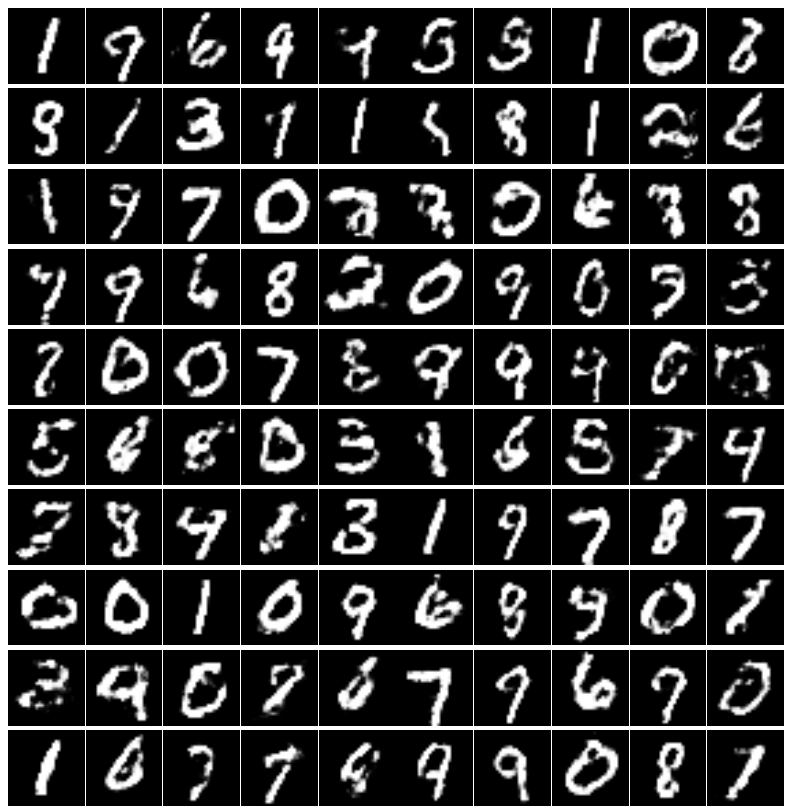
\includegraphics[scale=0.3]{images/generated.png}
\centering
\end{figure}

Our BiGRAN model, in contrast to a GRAN or GAN, is capable of autoencoding. Figure \ref{fig:autoencoded} shows samples from the true distribution, and several stochastic autoencodings of that sample.
 
\begin{figure}[h]
\caption{True samples (left column) and stochastic autoencodings of those samples.}
\label{fig:autoencoded}
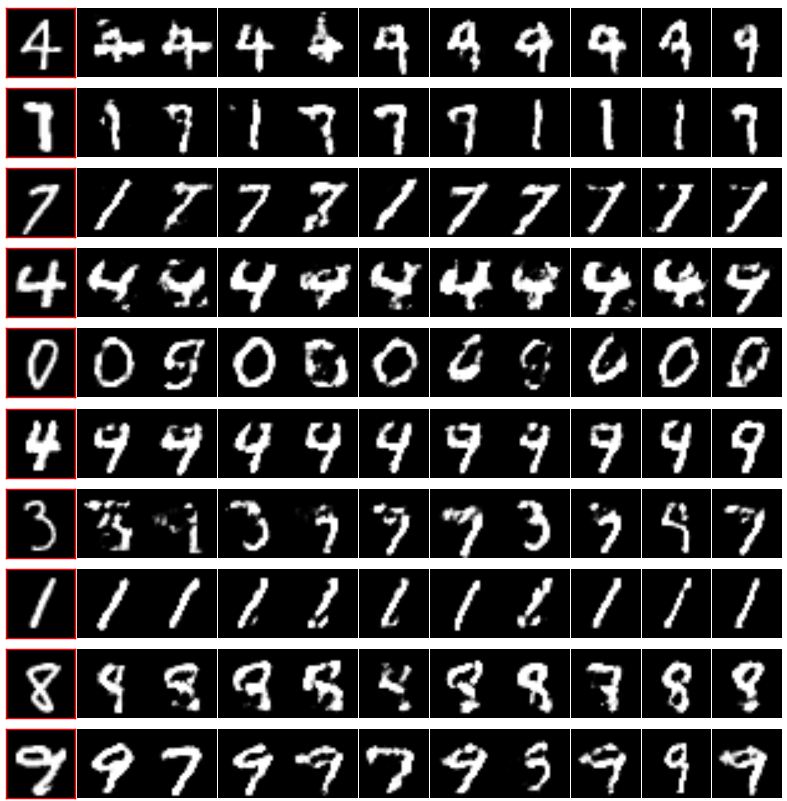
\includegraphics[scale=0.3]{images/autoencoding.png}
\centering
\end{figure}

Our model, in contrast to GANs and BiGANs, recurrently corrects the output and cumulatively draws the output image. In that sense, BiGRANs are to BiGANs as DRAW is to VAEs. As such, it would be natural to extend the BiGRAN with an attention mechanism. Without an attention mechanism, the BiGRAN can be seen to iteratively sharpen a blurry image, similar to results seen in DRAW without attention.

Figure \ref{fig:drawn} shows samples from the true distribution and how the canvas is iteratively constructed during autoencoding. The BiGRAN iteratively updates the canvas, building a sharper image from a blurrier image.
 
\begin{figure}[h]
\caption{True samples (left column) and the iterative generation of an autoencoding for those samples (recurrent depth = 4).}
\label{fig:drawn}
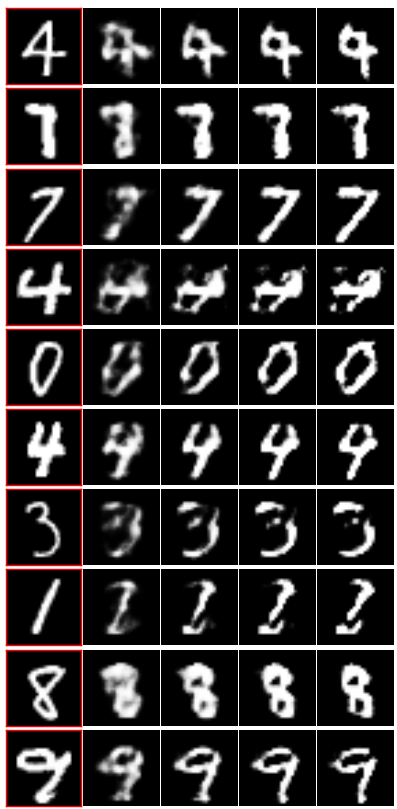
\includegraphics[scale=0.3]{images/drawing.png}
\centering
\end{figure}

 \section{Discussion}
 
BiGRANs provide a recurrent formulation for an autoencoder. However, instead of training an autoencoder to minimize mean squared error or some similar objective, it is trained to confuse a discriminator. The discriminator is then a novel form of objective function. Features of the discriminator, such as scale invariance due to convolution, mean that the objective of the generator has some scale invariance. Freedom from conventional objective functions enables more meaningful models. 

The recurrent formulation of BiGRANs allows for more expressive models, which would be further enhanced by methods of attention. Future work could include methods of attention and memory within a BiGAN or BiGRAN.

We found that without minibatch discrimination, GANs, including BiGRANs are prone to mode collapse. Recurrent discrimination appears to help avoid mode collapse, but complicated models such as BiGRANs can still enter into extended cycles.

Recurrent discrimination is one of the easiest ways to implement minibatch discrimination because it uses existing layers such as LSTMs. Iinformation goes through a hidden layer that bottlenecks to a constant width regardless of the depth of the LSTM. This may allow recurrent discrimination to scale more efficiently than other methods of minibatch discrimination.

There are many higher-level models that would be very interesting to explore given further advances in stabilizing GAN training. Methods such as unrolling \cite{DBLP:journals/corr/MetzPPS16} may be critical to preventing cycles. Future work should examine unrolling both discriminator and generator in combination with minibatch discrimination and other methods.

 GANs are sensitive to learning rates. Future research should include adaptive learning rates and attempting to determine the ideal relationship between the discriminator and generator learning rate.
 
%\medskip

\nocite{*}
\bibliography{bstriner_report}
\bibliographystyle{icml2016}

\end{document} 


% This document was modified from the file originally made available by
% Pat Langley and Andrea Danyluk for ICML-2K. This version was
% created by Lise Getoor and Tobias Scheffer, it was slightly modified  
% from the 2010 version by Thorsten Joachims & Johannes Fuernkranz, 
% slightly modified from the 2009 version by Kiri Wagstaff and 
% Sam Roweis's 2008 version, which is slightly modified from 
% Prasad Tadepalli's 2007 version which is a lightly 
% changed version of the previous year's version by Andrew Moore, 
% which was in turn edited from those of Kristian Kersting and 
% Codrina Lauth. Alex Smola contributed to the algorithmic style files.  
